\documentclass[hyperref={pdfpagelabels=false}]{beamer}

\usepackage{amssymb,amsthm,amsmath,mathrsfs,bm}

\renewcommand\refname{REFERENCE}
\setcounter{page}{1}



\newcommand{\defn}{\stackrel{\mbox{{\tiny def}}}{=}}
\newcommand{\trans}{^{\mbox{\tiny{T}}}}
\newtheorem{theo}{\bf Theorem}
\newtheorem{lemm}{\bf Lemma}

\def\I{{\bf I}}
\def\s{{\bf s}}
\def\b{{\bf b}}
\def\t{{\bf t}}
\def\x{{\bf x}}
\def\y{{\bf y}}
\def\m{{\bf m}}
\def\z{{\bf z}}
\def\calA{\mathcal{A}}
\def\calD{\mathcal{D}}
\def\calN{\mathcal{N}}
\def\calS{\mathcal{S}}
\def\wh{\widehat}
\def\wt{\widetilde}
\def\cov{\textrm{cov}}
\def\var{\textrm{var}}
\def\pr{\textrm{pr}}
\def\sp{\textrm{span}}
\def\tr{\textrm{tr}}
\def\dist{\textrm{dist}}
\def\vecl{\textrm{vecl}}
\def\eeqr{\end{eqnarray}}
\def\beqr{\begin{eqnarray}}
\def\eeqrs{\end{eqnarray*}}
\def\beqrs{\begin{eqnarray*}}
\def\bb{\mbox{\boldmath$\beta$}}
\def\ba{\mbox{\boldmath$\alpha$}}
%\def\be{\mbox{\boldmath$\eta$}}
\def\bGam{\mbox{\boldmath$\Gamma$}}
\def\blam{\mbox{\boldmath$\lambda$}}
\def\bLam{\mbox{\boldmath$\Lambda$}}
\def\bSig{\mbox{\boldmath$\Sigma$}}
\def\beps{\mbox{\boldmath$\varepsilon$}}
\def \hDash{\bot\!\!\!\bot}
\def\mR{\mathbb{R}}
\renewcommand{\baselinestretch}{1.25}

%------------In this paper----------------------------------
\newcommand{\M}{\mathbf{M}}
\newcommand{\bS}{\mathbf{S}}
\newcommand{\X}{\mathbf{X}}
\newcommand{\rl}{^{(l)}}
\newcommand{\iid}{\emph{i.i.d.}}
\newcommand{\diag}{\mathrm{diag}}
\newcommand{\trace}{\mathrm{trace}}
%\newcommand{\lE}{\mathbb{E}}
\newcommand{\lE}{{\rm{E}}}
\newcommand{\strans}{^{*\mbox{\tiny{T}}}}
\newcommand{\Col}{\mathrm{Col}}
\newcommand{\bP}{\mathbf{P}}
\newcommand{\bOm}{\mathbf{\Omega}}
\newcommand{\cU}{\mathcal{U}}
\newcommand{\bTh}{\mathbf{\Theta}}
\newcommand{\bPhi}{\mathbf{\Phi}}
\newcommand{\bXi}{\mathbf{\Xi}}
\newcommand{\bT}{\mathbf{T}}
\newcommand{\bG}{\mathbf{G}}
\newcommand{\SIR}{\mathrm{SIR}}
\newcommand{\CUME}{\mathrm{CUME}}
\newcommand{\Y}{\mathbf{Y}}
\newcommand{\ol}{\overline}
\newcommand{\rmI}{\mathrm{I}}
\newcommand{\bfa}{\mathbf{a}}
\newcommand{\be}{\mathbf{e}}
\newcommand{\tred}{\textcolor{red}}
\newcommand{\rmv}{{\rm{vec}}}
\newcommand{\bE}{\mathbf{E}}
\newcommand\independent{\protect\mathpalette{\protect\independenT}{\perp}}
\def\independenT#1#2{\mathrel{\rlap{$#1#2$}\mkern2mu{#1#2}}}
\def \O{O}
\def \o{o}
\newcommand{\B}{\mathbf{B}}
\newcommand{\bC}{\mathbf{C}}
\newcommand{\V}{\mathbf{V}}
\newcommand{\bv}{\mathbf{v}}
\newcommand{\bu}{\mathbf{u}}
\newcommand{\A}{\mathbf{A}}
\def\n{\nonumber}


%------------In this paper----------------------------------
\usepackage{url}
%% code from mathabx.sty and mathabx.dcl
%% for \widecheck
\DeclareFontFamily{U}{mathx}{\hyphenchar\font45}
\DeclareFontShape{U}{mathx}{m}{n}{
	<5> <6> <7> <8> <9> <10>
	<10.95> <12> <14.4> <17.28> <20.74> <24.88>
	mathx10
}{}
\DeclareSymbolFont{mathx}{U}{mathx}{m}{n}
\DeclareFontSubstitution{U}{mathx}{m}{n}
\DeclareMathAccent{\widecheck}{0}{mathx}{"71}
\DeclareMathAccent{\wideparen}{0}{mathx}{"75}

\def\cs#1{\texttt{\char`\\#1}}
% - widecheck

% Define

\newcommand{\cl}{\mathcal{l}}
\newcommand{\cL}{\mathcal{L}}
\def\sign{\textrm{sign}}
\newcommand{\bbeta}{\bm{\beta}}
\newcommand{\bvbeta}{\widecheck{\bbeta}}
\newcommand{\bhbeta}{\widehat{\bbeta}}
\newcommand{\btbeta}{\widetilde{\bbeta}}
\newcommand{\bbetaT}{{\bbeta^{\ast}}}
\newcommand{\bhSig}{\widehat{\bSig}}
\newcommand{\bvSig}{\widecheck{\bSig}}
\newcommand{\cH}{\mathcal{H}}
\newcommand{\argmin}{\mathop{\rm arg\min}}
\newcommand{\supp}{\mathrm{supp}}
\def\Z{{\bf Z}}
\def\vz{{\check{\z}}}
\def\hz{{\hat{\z}}}
\newcommand{\cC}{\mathcal{C}}
\newcommand{\op}{\mathrm{op}}
\newcommand{\pool}{\mathrm{pool}}
\newtheorem{remark}{\bf Remark}
% norm
\newcommand{\norm}[1]{\Vert#1\Vert}
\newcommand{\Norm}[1]{\left\Vert#1\right\Vert}
\newcommand{\inner}[2]{\langle #1, #2 \rangle}
\newcommand{\Inner}[2]{\left\langle #1, #2 \right\rangle}
\newcommand{\abs}[1]{\vert#1\vert}
\newcommand{\Abs}[1]{\left\vert#1\right\vert}

\newtheorem{prop}{\bf Proposition}
\newcommand{\bmu}{\bm{\mu}}
\newcommand{\tY}{\widetilde{\Y}}
\usepackage{float}
\usepackage[caption = false]{subfig}

% \usepackage{lmodern}
\usetheme{Frankfurt}
\title{A Two-stage Subgroup Analysis}  
\author{Chen Canyi} 
\date{\today} 
\begin{document}
% \logo{\includegraphics[scale=0.14]{logo-SF}}
\begin{frame}
\titlepage
\end{frame} 


\begin{frame}
\frametitle{Table of contents}
\tableofcontents
\end{frame} 


\section{Introduction} 
\begin{frame}
	\frametitle{Introduction} 
	\begin{itemize}
		\item Biological heterogeneity is common in many diseases.
		\item Thus there have been many attempts to identify subgroups from a heterogenous population.
		\item One of the most popular methods for finding subgroups from a heterogenous population is the mixture model.
	\end{itemize}
\end{frame}

\begin{frame}
	\frametitle{The mixture model}
\begin{itemize}
	\item need specify the underlying distribution for data
	\item the number of subgroups
	\item not suitable for the high dimensional setting $p>>n$, which is a common situation in precision medicine with high dimension genetic covariates $p$ and relative small sample size $n$.
\end{itemize}
\end{frame}

\section{Model}

\begin{frame}
	\frametitle{The model}
\begin{itemize}
	\item 	In this project, we consider the following model:
	\begin{eqnarray*}
	Y_{i} = \mu_{i} + \x_{i}\trans\bbeta + \epsilon_{i}, i = 1,\ldots,n,
	\end{eqnarray*}
	where $Y_i$ is the response for the $i$-th subject, $\mu_i$'s are unknown subject-specific intercepts.
	\item We assume the sparsity structure where only a subset $\calS$ of $\bbeta$ is nonzero. We assume $|\calS|=s$. 
\end{itemize}
\end{frame}

\begin{frame}
	\frametitle{Historical literature}
	\begin{itemize}
		\item In the situation $p<n$, Ma and Huang (2015) considered optimizing the following objective fucntion 
		$$
		Q_n(\bmu,\bbeta;\lambda) = 1/2\sum_{i = 1}^n(Y_i - \mu_i-\x_i^T\bbeta)^2 + \sum_{1\leq i<j\leq n} p(|\mu_i-\mu_j|,\lambda).
		$$
		\item alternating direction method of multipliers (ADMM) algorithm: a first order algorithm.
	\end{itemize}
\end{frame}

\begin{frame}
	\frametitle{Historical literature (Cont.)}
A nature extension to $p>n$
		\beqrs
		\widetilde{Q}_n(\bmu,\bbeta;\lambda) = 1/2\sum_{i = 1}^n(Y_i - \mu_i-\x_i^T\bbeta)^2 + \alpha_1\sum_{1\leq i<j\leq n} p(|\mu_i-\mu_j|,\lambda) \\+ \alpha_2 p(|\bbeta|,\omega).
		\eeqrs
		
		ADMM has to iterate on at lease ${n \choose 2} + p$ parameters sequentially.
\end{frame}

\section{Algorithm}
\begin{frame}
	\frametitle{The algorithm}
	\begin{itemize}
		\item Instead we first use Lasso procedure to select related covariates from $\x_i$, then apply k-means algorithm to the adjusted $\widetilde{Y_i}$. For the Lasso procedure, we minizize the following objective function
		\begin{equation}\label{eq:lasso}
		(\widehat{\mu}(\lambda),\widehat{\bbeta}(\lambda)) = \argmin_{(\mu,\bbeta)\in\mR^{p+1}} 1/2\sum_{i = 1}^n(Y_i - \mu-\x_i^T\bbeta)^2 + p(\bbeta,\lambda). 
		\end{equation}
		\item $\widetilde{Y_i} = Y_i - \x_i^T\widehat{\bbeta}$
	\end{itemize}
\end{frame}

\begin{frame}
	\frametitle{Choice of concave penalty function}
	\begin{itemize}
		\item $\ell_1$-norm penalty (Tibshirani, 1996, LASSO),
		smoothly clipped absolute deviations penalty (Fan and Li, 2001, SCAD) or minimax concave penalty (Zhang,
		2010, MCP).
		\item our choice: $p(\bbeta,\lambda) = \lambda|\bbeta|_1$.
	\end{itemize}
\end{frame}

\begin{frame}
	\frametitle{Optimization methods}
	\begin{itemize}
		\item The first order methods, such as Combettes and Pesquet (2011), Bach et al. (2012) and Tropp and Wright
		(2010), and Newton type algorithms, such as Fountoulakis et al. (2014) and Dassios et al. (2015), can be used
		to optimize (1).
		\item We suggest to use the primal dual active set method (Fan et al., 2014), which is in spirit a
		generalized version of Newton type method. It usually converges after one-step iteration if there is a very
		good initial value.
	\end{itemize}
\end{frame}

\begin{frame}
	\frametitle{The remains: One-dimension cluster}
	\begin{itemize}
		\item It remains to analysis the subgroups in $\tY = (\widetilde{Y_1},\ldots,\widetilde{Y_n})^T$.
		\item e.g., k-means, k-median, k-modes, even the deep learing algorithm.
		\item It is NP-hard in a general Euclidean space, even when the number of clusters k is 2  (Aloise et al., 2009).
		\item optimal one-dimensional clustering: $O(qknp)$ v.s. $(kn lg n)$ 
	\end{itemize}
\end{frame}

\begin{frame}
	\frametitle{Selection of the tuning parameters $k$ and $\lambda$}
	\begin{itemize}
		\item We select the tuning parameter $\lambda$ by validation.
		\item Bayesian Information Criterion
		$$
		\mathrm{BIC}(k) = \log \left[\sum_{i = 1}^n\{Y_i - \widehat{\mu_i}(k) - \x_i^T\widehat{\bbeta}\}^2/n\right] + C_n \log n/n(k + s),
		$$
		where $C_n = c\log\{\log(n+s)\}$ with some positive constant $c$. We take $c = 10$ by defaults.
	\end{itemize}
\end{frame}

\section{Emperical Example}
\begin{frame}
	\frametitle{Chemores Data Example}
	\begin{itemize}
		\item Lung cancer is one of the most prevalent and deadiest cancers, which can be classified into two major subtypes,
		small cell lung cancer (SCLC) and non-small cell lung cancer (NSCLC). NSCLC accouting 80% of all primary
		lung cancers, is a known heterogeneous group and its prognosis is generally poor (Tsuboi et al., 2007).
		\item Publicly available lung cancer genomic data from the Chemores Cohort Study. This data is part of an integrated study of mRNA, miRNA and clinical variables to characterize the molecular distinctions between squamous cell carcinoma (SCC) and adenocarcinoma (AC) in Non Small Cell Lung Cancer (NSCLC) aside large cell lung carcinoma (LCC).
	\end{itemize}
\end{frame}

\begin{frame}
	\frametitle{Results}
		\begin{columns}[t]
			\column{.5\textwidth}
			\centering
			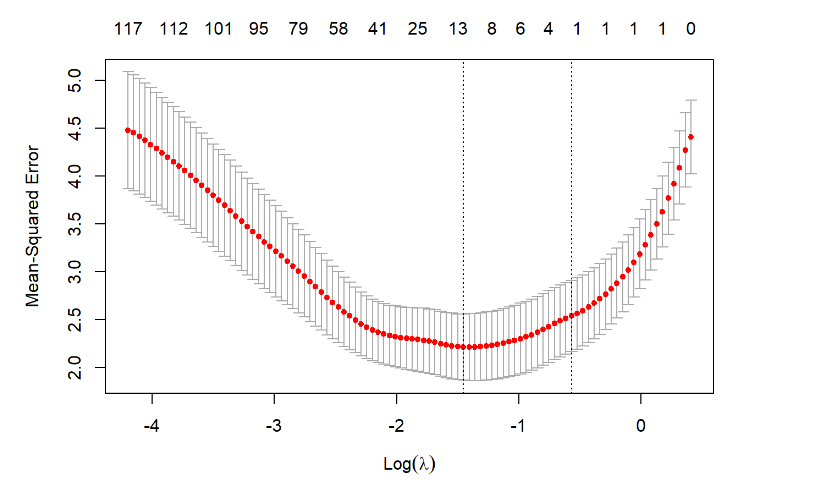
\includegraphics[width = \textwidth]{fig/ChenCV.png}\\
			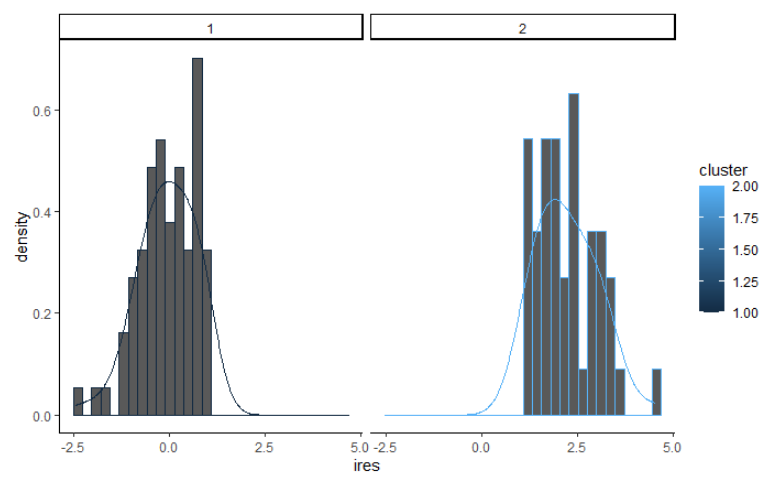
\includegraphics[width = \textwidth]{fig/ChenOnemode.png}
			\column{.5\textwidth}
			\centering
			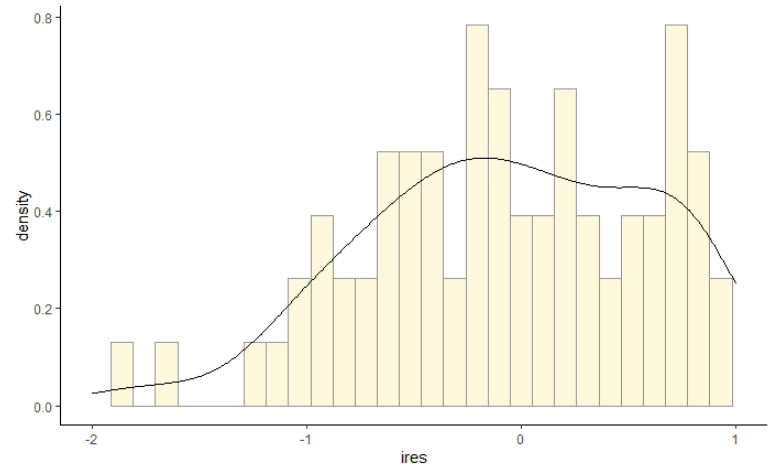
\includegraphics[width = \textwidth]{fig/ChenTwomode.png}\\
			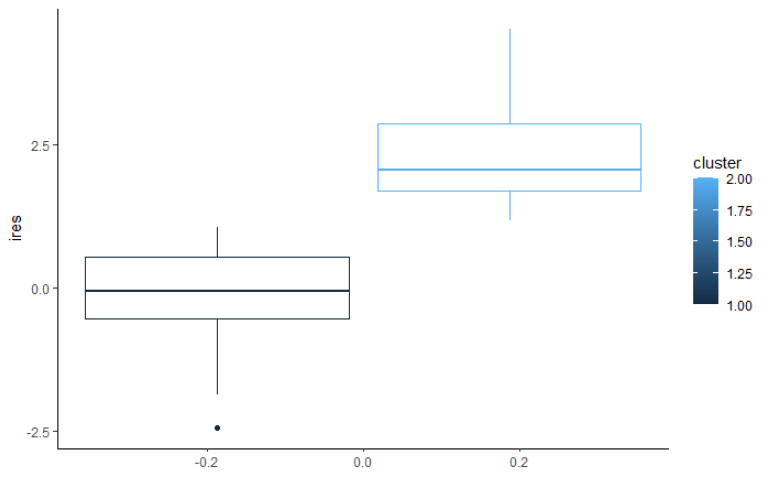
\includegraphics[width = \textwidth]{fig/ChenBox.png}
		\end{columns}
\end{frame}

\begin{frame}
	\frametitle{Results}
		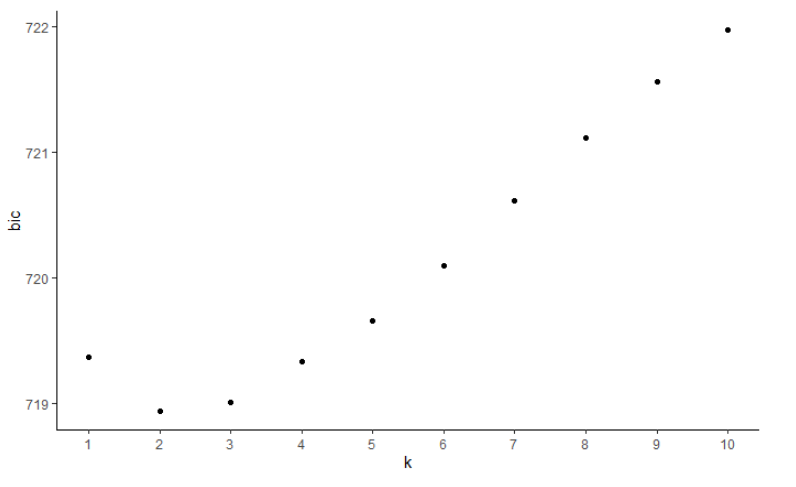
\includegraphics[width = \textwidth]{fig/ChenBic.png}\\

\end{frame}

\end{document}


